\chapter{Splitting the Assembly Map}\label{c7}

Between\pageoriginale the notions of normal cobordism on a manifold
$M$ and special normal cobordism on $M$, there is an intermediate
object called a \textit{simple} normal cobordism. Recall that a normal
cobordism on $M$ is a triple $(W, F, \simeq)$ in which $F$ is a map
$F: W \to M \times I$ such that $F|_{\partial +w}: \partial^+ W \to M
\times 1$ is a homotopy equivaoence and $F|_{\partial ^- W}: \partial
^- W \to M \times 0$ is the identity map. If $F|_{\partial^+ W}:
\partial^+ W \to  M \times 1$ is a simple homotopy equivalence, we say
that $(W, F, \simeq)$ is a \textit{simple normal cobordism}. (Recall
that $(W, F, \simeq)$ is a special normal cobordism if $F|_{\partial
  ^+ W}$ is a homeomorphism.) There is an obvious equivalence relation
on the set of simple normal cobordisms analogous to the equivalence
relation on normal cobordisms and special normal cobordisms. Wall
\cite{96} showed that the equivelence classes of simple normal
cobordisms form an abelian group, denoted by $L^s_{m+1} (\pi_1 M)$,
which depends only on $\pi_1 M$ and on the first Stiefel-Whitney class
$w_1 (M)$. The forget structure maps define group homomorphisms
\begin{align*}
  \ob{\sigma} & : [M \times [0,1], \partial; G/\ttop]\to
  L^s_{m+1} (\pi_1 M) ~\text{and}\\
\eta & : L_{m+1}^s (\pi_1 M) \to L_{m+1} (\pi_1 M).
\end{align*}

And these homomorphisms factor the assembly map
$$
\sigma : [M \times [0, 1], \partial; G/\ttop]\to L_{m+1}(\pi_1 M)
$$
as $\sigma = \eta \circ \ob{\sigma}$. It is known that $\eta$ is in
isomorphism after tensoring with $\mathbb{Z}[1/2]$. This is a
consequence of Rothenberg's exact sequence, cf. \cite[p. 248]{96}. Of
course $\eta$ is an isomorphism before tensoring with $Z[1/2]$ if $Wh
(\pi_1 M)=0$. 

Recall condition $(*)$ defined in Lecture \ref{c6}. Farrell and Hsiang
\cite{30} split the simple assembly map when $M$ satisfies condition
$(*)$. The precise statement is the following.

\begin{thm}\label{c7:thm7.1}
  Let $M^m$ be a closed manifold satisfying condition $(*)$ and let
  $\ob{\sigma} : [M \times \mathbb{D}^n, \partial; G/\ttop]\to
  L_{n+m}^s(\pi_1 M)$ be the simple assembly map. Then $\ob{\sigma}$
  is a split monomorphism provided $n \geq 2$ and $n+ m \geq 7$.
\end{thm}

\begin{proof}
  In\pageoriginale order not to obscure the main idea of the proof, we
  will assume that $M$ is triangulated and that $n=2$. We will
  construct a function
  $$
  d: L_{m+2}^s (\pi_1 M)\to [M^m \times \mathbb{D}^2, \partial; G/\ttop]
  $$
  such that $d \circ \ob{\sigma} = id$. This shows that $\ob{\sigma}$
    is a monomorphism. We will not verify that $d$ is a group
    homomorphism since this will not be important to our later
    applications of Theorem \ref{c7:thm7.1}.
\end{proof}

To construct $d$, we will use the geometric description of
$\ob{\sigma}$ as the forget structure map from the equivalence classes
of special normal cobordisms on $M \times [0,1]$ to the equivalence
classes of simple normal cobordisms on $M \times [0, 1]$. Hence, given
a simple normal cobordism $(W, F, \simeq)$ on $M \times [0,1]$, $I$ must
give a method which produces a special normal cobordism $(W', F',
\simeq')$ on $M \times [0, 1]$ in such a way that if $(W, F, \simeq)$
is already special, then $(W', F', \simeq')= (W, F, \simeq)$.

Since $M$ satisfies condition $(*)$, identify the deck transformation
action of $\pi_1 (M)$ on $\tilde{M}$ with the action of $\pi_1(M)$ on
Int $(\mathbb{D}^m)$ mentioned in the definition of condition
$(*)$. The action of $\pi_1 (M)$ on $\mathbb{D}^m$ naturally extends
to an action of $\pi_1 (M)$ on $\mathbb{D}^{m+1}$ as indicated in
Figure 4.

\begin{figure}[H]
  \centering{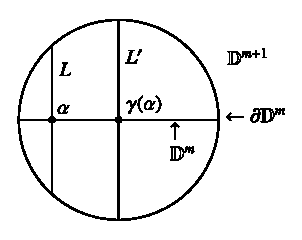
\includegraphics{vol86-figures/fig4.eps}\\
  Figure 4\qquad }
\end{figure}

Here, the action of $\gamma \in \pi_1(M)$ linearly maps the vertical
line segment $L$ in $\mathbb{D}^{m+1}$ which meets $\mathbb{D}^m$
perpendicularly in the point $x$ to the vertical line segment $L'$
meeting $\mathbb{D}^m$ at $\gamma (x)$. Notice that the extended
action satisfies the following analogues of properties 1 and 2 of
condition $(*)$.

\begin{enumerate}[$1.'$]
\item The\pageoriginale restriction of the action of $\pi_1 (M)$ to
  $\mathbb{D}^{m+1}- \partial \mathbb{D}^m$ is equivalent to the deck
  transformation action on the universal cover of $M \times [0,1]$.
  \item Given $\epsilon > 0$ and a compact subset $K$ of
    $\mathbb{D}^{m+1}- \partial \mathbb{D}^m$, there exists a number
    $\delta > 0$ such that the following is true for every $\gamma \in
    \pi_1 (M)$. If the distance between $\gamma K$ and $\partial
    \mathbb{D}^m$ is less than $\delta$, then diam $(\gamma K)< \epsilon$. 
\end{enumerate}

Again identify the action of $\pi_1(M)$ on $\tilde{M} \times [0,1]$
with the extended action of $\pi_1(M)$ on $\mathbb{D}^{m+1}-\partial
\mathbb{D}^m$. Now properties $1'$ and $2'$ have the following
important consequence $(**)$.

\begin{itemize}
\item[$(**)$] Let $h: M \times I \to M \times I$ be any self-map with
  $h|_{M \times 0}= id_{M \times 0}$. Then its unique lift $\tilde{h}
  : \tilde{M}\times I \to \tilde{M} \times I$, with
  $\tilde{h}|_{\tilde{M}\times 0}= id_{\tilde{M} \times 0}$, uniquely
  extends to a self map $\tilde{h} : \mathbb{D}^{m+1} \to
  \mathbb{D}^{m+1}$ by setting $\tilde{h}|_{\partial \mathbb{D}^m}=
    \text{id}_{\partial \mathbb{D}^m}$.
\end{itemize}

For the remainder of the proof, let $\Gamma$ denote $\pi_1(M)$. Note
that the extension $\tilde{h}$ of $(**)$ is a $\Gamma$-equivariant
map. Since the universal cover $\tilde{M} \to M$ is a principal
$\Gamma$-bundle, we can form the associated $\mathbb{D}^{m+1}$-bundle
$\tilde{E} \to M$ whose total space is $\tilde{M} \times \Gamma
\mathbb{D}^{m+1}$; i.e., $\tilde{E}$ is the orbit space of the
diagonal action of $\Gamma$.

The action of $\Gamma$ on $\mathbb{D}^{m+1}$ leaves invariant the
northern and southern hemispheres of $\partial \mathbb{D}^{m+1}$;
which we denote by $\partial_+ \mathbb{D}^{m+1}$ and $\partial_-
\mathbb{D}^{m+1}$, respectively. It also leaves invariant the equator
$\partial \mathbb{D}^m$. (See Figure 5.) 
\begin{figure}[H]
  \centering{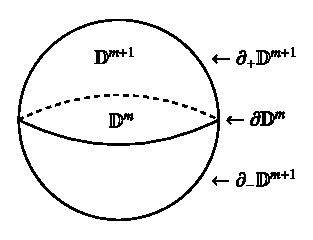
\includegraphics{vol86-figures/fig5.eps}\\
    Figure 5\qquad }
\end{figure}

The associated $\partial_+ \mathbb{D}^{m+1}$, $\partial_-
\mathbb{D}^{m+1}$ and $\partial \mathbb{D}^m$-bundles to $\tilde{M}
\to M$ are sub-bundles of $\ob{E} \to M$.\pageoriginale Their total spaces are
denoted by $\partial _+ \ob{E}$, $\partial_- \ob{E}$ and $\partial _0
\ob{E}$, respectively. 

Let $(W, F \simeq)$ be a simple normal cobordism on $M \times I$. (See
Figure 6).
\begin{figure}[H]
  \centering{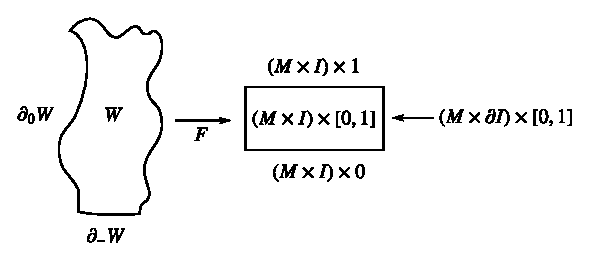
\includegraphics{vol86-figures/fig6.eps}\\
  Figure 6}
\end{figure}

Recall $\partial W = \partial_- W \cup \partial _+ W \cup \partial_0
W$ and $F|_{\partial W} = F_- \cup F_+ \cup F_0$, where
\begin{align*}
  F_- & : \partial _- w \to (M \times I) \times 0 ~\text{is the
    identity map};\\
  F_+ & : \partial_+ W \to (M \times I) \times 1 ~\text{is a simple
    homotopy equivalence};\\
  F_0 & : \partial_0 W \to (M \times \partial I) \times [0, 1]
  ~\text{is a homeomorphism}.
\end{align*}

Consequently, $\partial_+ W$ is an $s$-cobordism and hence a
cylinder. We can therefore identify $\partial _+ W$ with $M \times I= M
\times [0, 1]$ in such a way that $F_+ : M \times I \to M \times I$ is
a homotopy equivalence; $F_+|_{M \times 0} = id_{M \times 0}$ and
$F_+|_{M \times 1}$ is a self homeomorphism.
